\documentclass{article}
\usepackage{tikz}
\usepackage{skak} 
\usetikzlibrary{arrows,automata}
\usetikzlibrary{positioning}

\pagestyle{empty}

\begin{document}
Bill Davis\\
Homework 1

\begin{enumerate}
  \item[4]
  	\begin{enumerate}
    	\item[a]

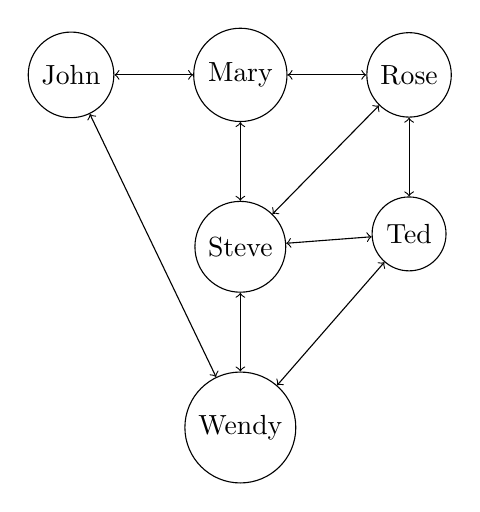
\begin{tikzpicture} [every node/.style={draw,circle}]
\node (a) {John};
\node (b) [right=of a] {Mary};
\node (c) [right=of b] {Rose};
\node (d) [below=of b] {Steve};
\node (e) [below=of c] {Ted}; 
\node (f) [below=of d] {Wendy};  

\draw[<->](a)--(b);
\draw[<->](a)--(f);
\draw[<->](b)--(c);
\draw[<->](b)--(d);
\draw[<->](c)--(d);
\draw[<->](c)--(e);
\draw[<->](d)--(e);
\draw[<->](d)--(f);
\draw[<->](e)--(f);      
\end{tikzpicture}   	
    	
    	\item[b]
    	Steve will hear the rumor in 1 day, from both Mary and Wendy. 
    	\item[c]
    	If (John and Mary) stop talking and (Wendy and Steve) stop talking, then
    	it would take three days to get from John to Mary (through wendy, ted,
    	steve).
      \end{enumerate} 
      
      \item[7] 
      There are three ways to get from A$\rightarrow$G. These are ABCEFG(1),
      ABEFG(2), and ABDFG(3), where the first one takes 6 steps and the other two take 5.
      There are then 3 ways to get from G$\rightarrow$B back to H, These are
      BCEFG(4), BEFG(5), and BDFG(6), where 4 takes 5 steps and 5,6 both take 4
      steps.
      
      So then in order to get to 15 steps, there are 4 ways to start with 1,
      (145,146,154,164), and 1 way that start with 2 (244) and 1 way that
      starts with 3 (344) for a total of 6 possible sequences of 15 steps.
      
      \item[12]
      \begin{enumerate}
      	\item[a]
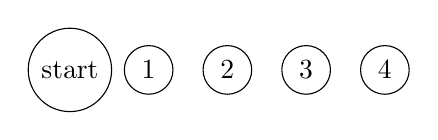
\begin{tikzpicture} [every node/.style={draw,circle}]
\node (start) {start};
    \foreach \i in {1,...,4}
    {
    	\node(\i)at (\i,0){\i}; 
    }    
\end{tikzpicture} 

		item[b]
				      
      		        
      \end{enumerate}
      
      \item[18]
      \begin{enumerate}
      \item[a]
      The removal of the following pairs will disconnect the graph, (c,e),
      (b,g), (b,f), (c,f), (d,f)
      \item[b]
      The removal of the following sets of edges will disconnect the graph,
      (ab,ag),(cd,de), (de,ef),  
      \item[c]
      The minimum number of vertices that need to be removed to disconnect the
      graph of the 12 edges of a cube is 3. 
      \end{enumerate}
      
      \item[21]
      \begin{enumerate}
              \item[a]
              
              \newgame
   \fenboard{7q/6q1/5q2/8/3q4/2q5/1q6/q7
   w - - 0 20}

              \showboard
              \item[b]
      \end{enumerate}
      \item[23]
      
      \item[36]
\end{enumerate}

\begin{center}


\begin{tikzpicture}[every node/.style={draw,circle}]
\begin{scope}[node distance=5mm]
	\node(a) at (1,1) {a};
\end{scope}
\end{tikzpicture}

here is more

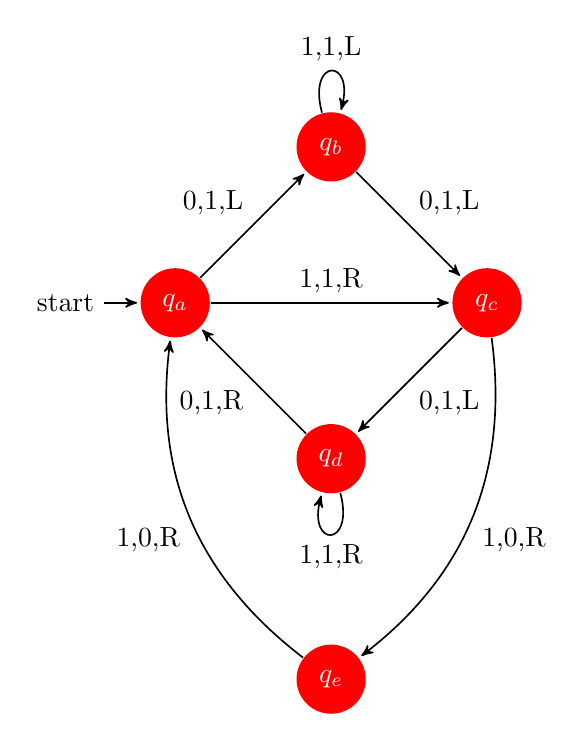
\begin{tikzpicture}[->,>=stealth',shorten >=1pt,auto,node distance=2.8cm,
                    semithick]
  \tikzstyle{every state}=[fill=red,draw=none,text=white]

  \node[initial,state] (A)                    {$q_a$};
  \node[state]         (B) [above right of=A] {$q_b$};
  \node[state]         (D) [below right of=A] {$q_d$};
  \node[state]         (C) [below right of=B] {$q_c$};
  \node[state]         (E) [below of=D]       {$q_e$};

  \path (A) edge              node {0,1,L} (B)
            edge              node {1,1,R} (C)
        (B) edge [loop above] node {1,1,L} (B)
            edge              node {0,1,L} (C)
        (C) edge              node {0,1,L} (D)
            edge [bend left]  node {1,0,R} (E)
        (D) edge [loop below] node {1,1,R} (D)
            edge              node {0,1,R} (A)
        (E) edge [bend left]  node {1,0,R} (A);
\end{tikzpicture}



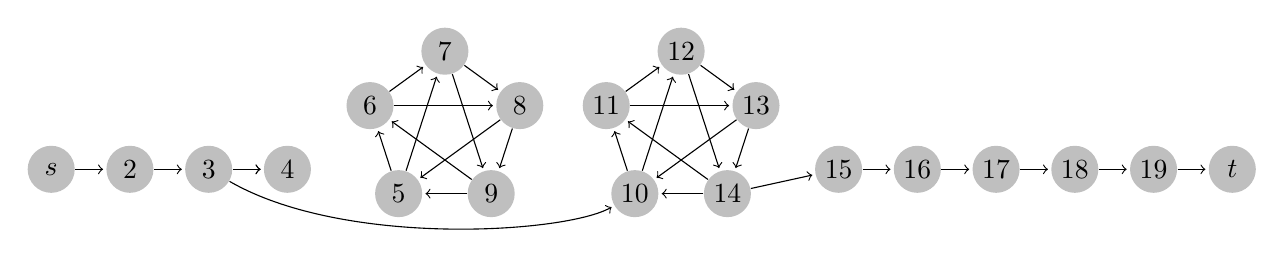
\begin{tikzpicture}[shorten >=1pt,->]
  \tikzstyle{vertex}=[circle,fill=black!25,minimum size=17pt,inner sep=0pt]

  \foreach \name/\x in {s/1, 2/2, 3/3, 4/4, 15/11, 
                        16/12, 17/13, 18/14, 19/15, t/16}
    \node[vertex] (G-\name) at (\x,0) {$\name$};

  \foreach \name/\angle/\text in {P-1/234/5, P-2/162/6, 
                                  P-3/90/7, P-4/18/8, P-5/-54/9}
    \node[vertex,xshift=6cm,yshift=.5cm] (\name) at (\angle:1cm) {$\text$};

  \foreach \name/\angle/\text in {Q-1/234/10, Q-2/162/11, 
                                  Q-3/90/12, Q-4/18/13, Q-5/-54/14}
    \node[vertex,xshift=9cm,yshift=.5cm] (\name) at (\angle:1cm) {$\text$};

  \foreach \from/\to in {s/2,2/3,3/4,3/4,15/16,16/17,17/18,18/19,19/t}
    \draw (G-\from) -- (G-\to);

  \foreach \from/\to in {1/2,2/3,3/4,4/5,5/1,1/3,2/4,3/5,4/1,5/2}
    { \draw (P-\from) -- (P-\to); \draw (Q-\from) -- (Q-\to); }

  \draw (G-3) .. controls +(-30:2cm) and +(-150:1cm) .. (Q-1);
  \draw (Q-5) -- (G-15);
\end{tikzpicture}

\end{center}
Here is text
\end{document}